\documentclass[12pt]{article}
\usepackage{enumitem}
%\usepackage[T1]{fontenc}
\usepackage[auth-sc,affil-sl]{authblk}
\usepackage{amsmath}
\usepackage{graphicx}
\usepackage{color}
\usepackage[toc,page]{appendix}
%\usepackage{enumerate}
\usepackage[round]{natbib}
%\usepackage{url} % not crucial - just used below for the URL 
%\usepackage{amsthm}
\usepackage{amssymb}
\usepackage{graphicx}
\usepackage{epstopdf}
\usepackage{hyperref}
\usepackage{alltt}
\usepackage{listings}
\usepackage{array}
\usepackage[noline, boxed, linesnumbered, procnumbered, titlenumbered]{algorithm2e}
%\usepackage[firstpage]{draftwatermark}
\usepackage[margin=1in]{geometry}  %%jcgs has own margins
\usepackage{lmodern}
\usepackage{caption}
\usepackage{subcaption}

%\pdfminorversion=4
% NOTE: To produce blinded version, replace "0" with "1" below.
\newcommand{\blind}{0}

\newcommand{\secref}[1]{Section~\ref{#1}}
\newcommand{\appdxref}[1]{Appendix~\ref{#1}}
\newcommand{\tblref}[1]{Table~\ref{#1}}
\newcommand{\figref}[1]{Figure~\ref{#1}}
\newcommand{\thmref}[1]{Theorem~\ref{#1}}
\newcommand{\algref}[1]{Algorithm~\ref{#1}}
\newcommand{\funref}[1]{Function~\ref{#1}}
\newcommand{\listingref}[1]{Listing~\ref{#1}}

\newcommand{\eg}{{\em e.g.}}
\newcommand{\ith}{$i^{th}$}
\newcommand{\cut}[1]{}
\newcommand{\todo}[1]{{{\color{red}{[#1]}}}}

\newcommand{\Ex}{\mathop{\mathbb{E}}}
\newcommand{\Imp}{\mathbf{I}}

\newcommand{\spd}{\fontfamily{cmr}\textsc{\small StratPD}}
\newcommand{\cspd}{\fontfamily{cmr}\textsc{\small CatStratPD}}
\newcommand{\xnc}{$x_{\overline{c}}$}
\newcommand{\xnC}{$x_{\overline{C}}$}

\setlist[enumerate]{itemsep=-1mm}

% DON'T change margins - should be 1 inch all around.
\cut{
\addtolength{\oddsidemargin}{-.5in}%
\addtolength{\evensidemargin}{-.5in}%
\addtolength{\textwidth}{1in}%
\addtolength{\textheight}{1.3in}%
\addtolength{\topmargin}{-.8in}%
}

\begin{document}

\def\spacingset#1{\renewcommand{\baselinestretch}%
{#1}\small\normalsize} \spacingset{1}


%%%%%%%%%%%%%%%%%%%%%%%%%%%%%%%%%%%%%%%%%%%%%%%%%%%%%%%%%%%%%%%%%%%%%%%%%%%%%%

\if0\blind
{
  \title{\bf Model-Free Feature Importance}

  \author{Terence Parr and James D. Wilson\\
      University of San Francisco\\
}
  \maketitle
} \fi

\if1\blind
{
  \bigskip
  \bigskip
  \bigskip
  \begin{center}
    {\LARGE\bf Title}
\end{center}
  \medskip
} \fi

\bigskip
\begin{abstract}
dsf
\end{abstract}

\noindent%
{\it Keywords:} feature importance, partial dependence, model interpretability, linear models
%\vfill

%\newpage
%\spacingset{1.5} % DON'T change the spacing!
\section{Introduction}
\label{sec:intro}

Among data analysis techniques, feature importance is one of the most  useful. Data science practitioners use feature importance to gain business insights (e.g., identifying product characteristics valued by customers) and to select features for predictive models (dropping the least predictive features to simplify and potentially increase the generality of the model). While some approaches work directly on the data, such as principle component analysis (PCA), the vast majority of feature importance algorithms analyze data through the lens of a specific model fitted to the data, or even through subsidiary models to analyze such fitted models (LIME, SHAP, permutation, drop column).

Relying on a fitted model introduces a number of issues. First, practitioners must choose an appropriate model that captures the relationship between features and target; inaccurate models do not yield useful feature importance results. But, more importantly, it is possible to get very different feature importances running the same algorithm on the same data, just by choosing a different model. This fact should reduce trust in algorithms operating on fitted models. consider the example in \figref{fig:diff-models}

\begin{figure}[htbp]
\begin{center}
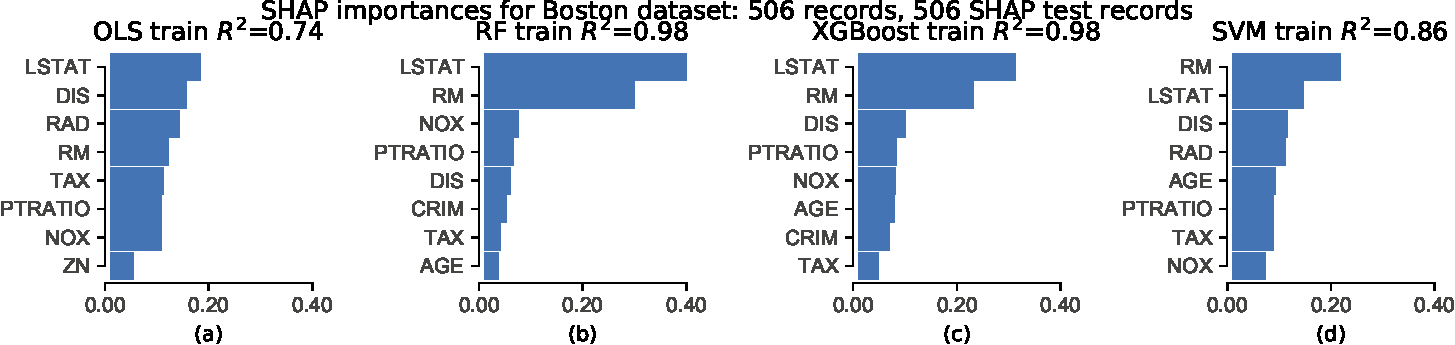
\includegraphics[scale=0.54]{images/diff-models.pdf}
\caption{foobar. \texttt{\footnotesize RandomForestRegressor(n\_estimators=30)}, \texttt{\footnotesize XGBRegressor(max\_depth=5, eta=.01, n\_estimators=50)} }
\label{fig:diff-models}
\end{center}
\end{figure}

btw, SHAP claims to be model independent but it?s not usable in that configuration.  only linear and tree explainers complete in our lifetime and they exploit details of linear models and trees to go fast hence NOT independent

people focus on "intersting features" but spurious OR function of model not data.

\section{foo}

For true function $y = f(\bf x)$ and ${\bf x} = [x_1, \ldots, x_p]$ and ${\bf X} = [x^{(1)}, \ldots, x^{(n)}]$ (skipping bolding the vectors there).  Training data is pair ($\bf X, y$).

The partial dependence of $y$ on  $x_i$ is the isolated contribution of $x_i$ to $y$. At some $x_j=z$ value, the partial dependence is the cumulative sum of $\frac{\partial y}{\partial x_j}$ from $min(x_j)$ up to $z$:

\[
\text{\it PD}_j(z) = \int_{min(x_j)}^z \frac{\partial y}{\partial x_j} dx_j
\]

Software currently relies on something like:

\[
\Ex[\text{\it PD}_j] = \frac{1}{N} \sum_{i=1}^{N} \text{\it PD}_j(x_j^{(i)})
 \]

\[
\Imp_j = \Ex[|\text{\it PD}_j|]
\]

or normalized 0..1 as:

\[
\Imp_j = \frac{\Ex[|\text{\it PD}_j|]}{\Ex[y]}
\]

\noindent where

\[
\Ex[y] = \sum_{j=1}^p \Ex[\text{\it PD}_j]%\big |_{min(x_j)}^{max(x_j)}
\]

or, with less accurate PDP (to keep 0..1) since

\[
\Imp_j = \frac{\Ex[|\text{\it PD}_j|]}{\sum_{k=1}^p \Ex[|\text{\it PD}_k|]}
\]

\bibliographystyle{apalike}

\bibliography{stratpd}
\end{document}